%!TEX root = ../Report.tex
%************************************************

% Results

\chapter{Results}

\section{Introduction}
This chapter outlines the results, including the design of the user interface, functionality of the application and a short summary of the results of the incorporated algorithms.
The majority of the results have already been covered in part \ref{part:algo}, however a discussion is provided.

\section{User interface}

\begin{figure}
\centerline{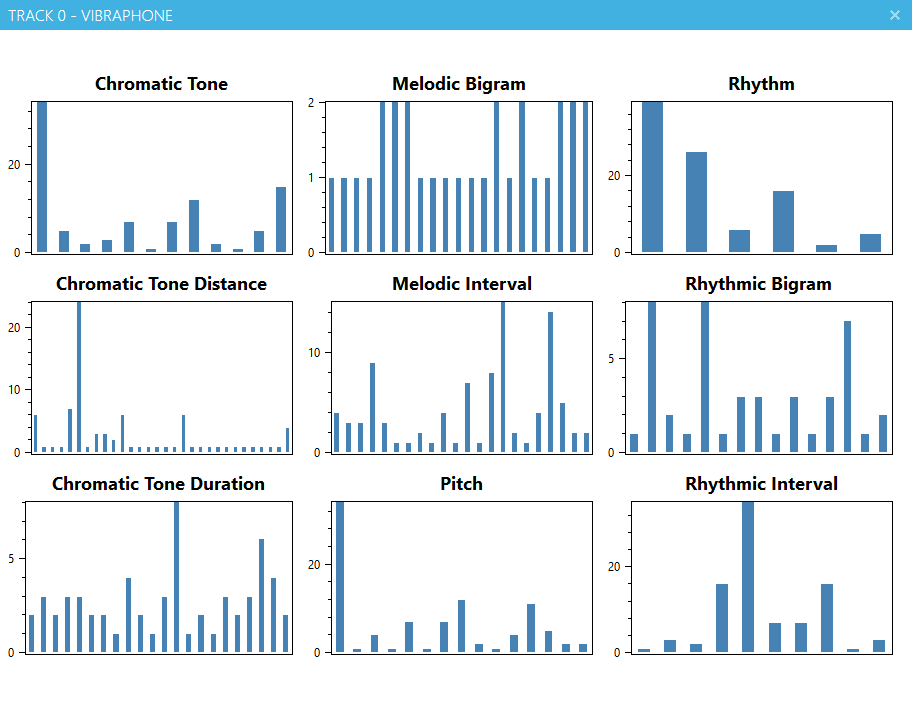
\includegraphics[width=300px]{../images/res_ui_metrics_harry_t0.png}}
\caption{Frequency metrics for the first track Harry Potter Opening Theme Song}
\label{ims:metricsharryt0}
\end{figure}

Figure \ref{ims:metricsharryt0} shows the frequency metrics for the first track of the Harry Potter opening theme song.

\begin{figure}
\centerline{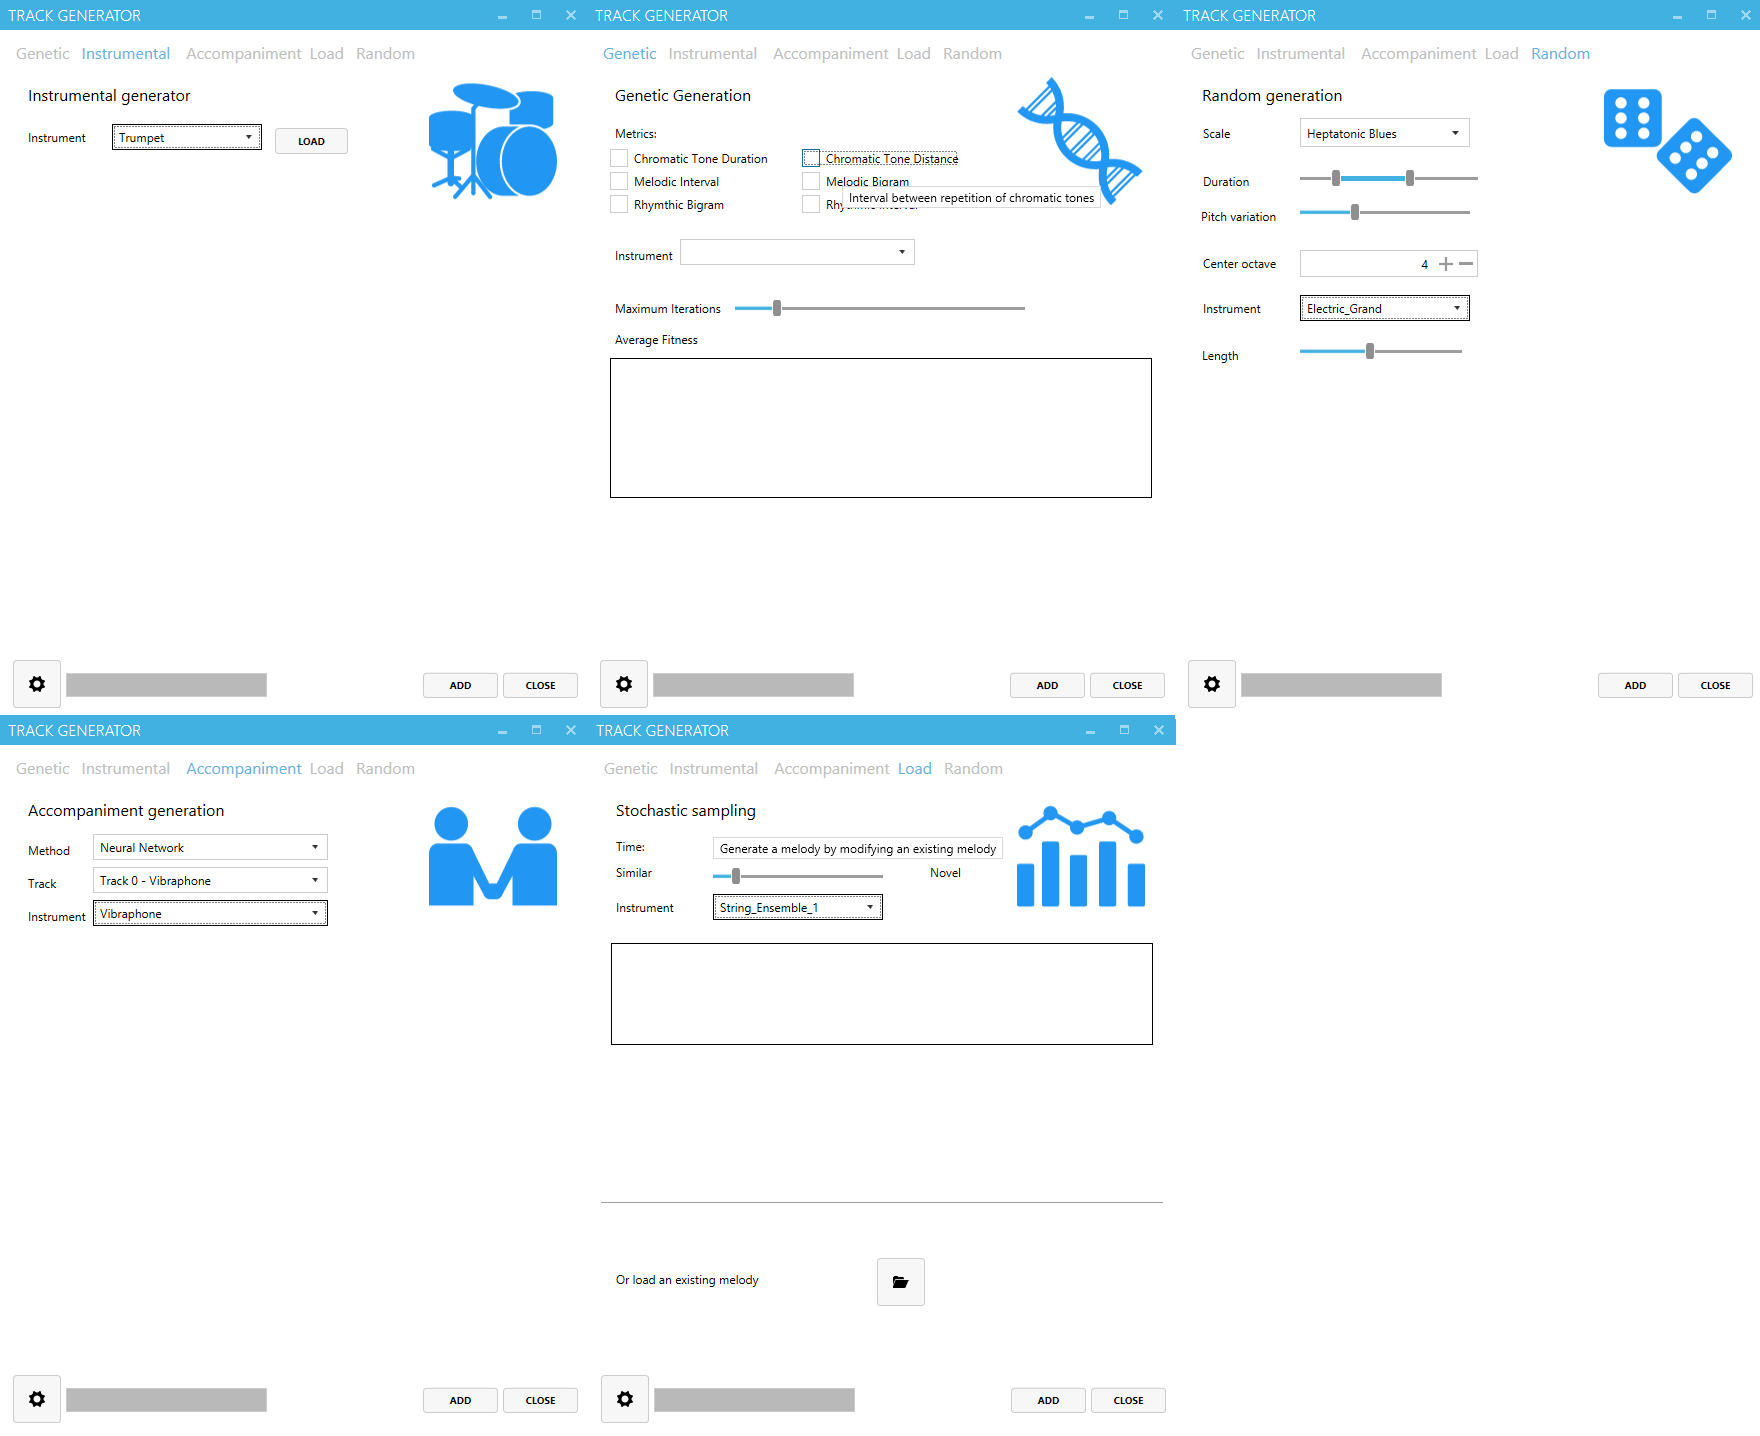
\includegraphics[width=400px]{../images/ui_trackgen_alltabs.png}}
\caption{Tabs of the track generator window}
\label{ims:uitrackgenalltabs}
\end{figure}

Figure \ref{ims:uitrackgenalltabs} shows the track generator with all of the available tabs.
These tabs provide the following features:
\begin{enumerate}
\item Genetic - Generates a melody using genetic algorithm. Allows selection of which frequency metrics to use with the cosine similarity fitness function.
\item Instrumental - Generates a melody using Markov Chains for a particular instrument.
\item Accompaniment - Generates a accompaniment melody for a main melody track using a Markov model or a \ac{ANN}.
\item Load - Loads an existing melody or modifies an extant melody using stochastic sampling
\item Random - Generates a random melody using a random walk in a specific scale.
\end{enumerate}

\begin{figure}
\centerline{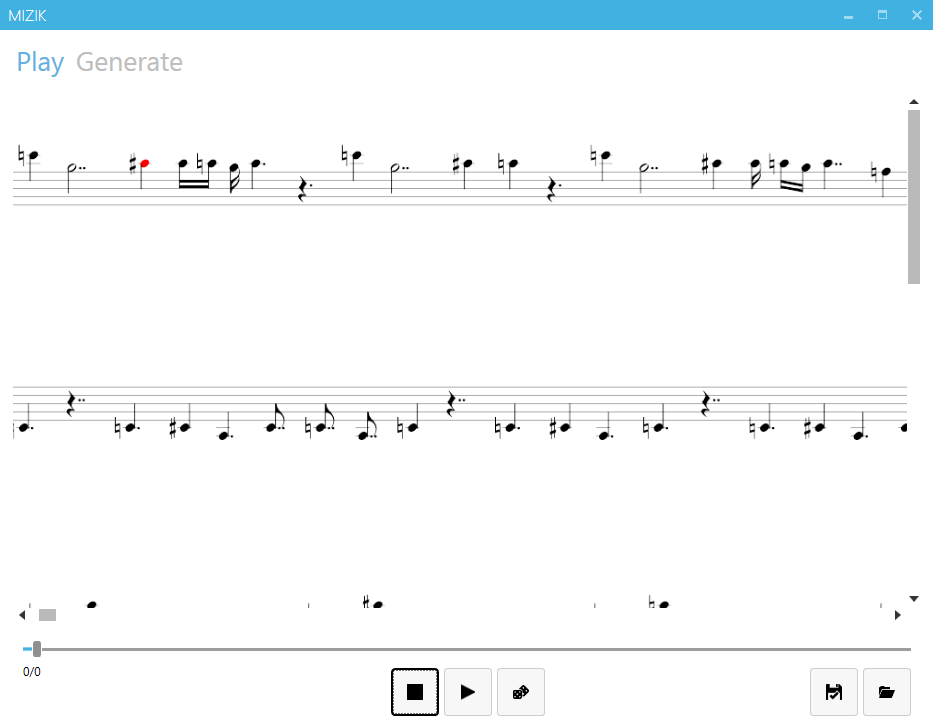
\includegraphics[width=400px]{../images/res_ui_playback.png}}
\caption{Playback tab of main window}
\label{ims:res_ui_playback}
\end{figure}

Figure \ref{ims:res_ui_playback} shows the play tab of the main window. The play tab offers access to all playback functionality including playing, stopping and seeking the position of a melody.
In addition the play tab allows the user to re-randomize the melody. The current melody can be saved or an existing melody can be loaded.
Lastly the play tab shows a visualization of the current song playing. A note being played is highlighted in red.

\begin{figure}
\centerline{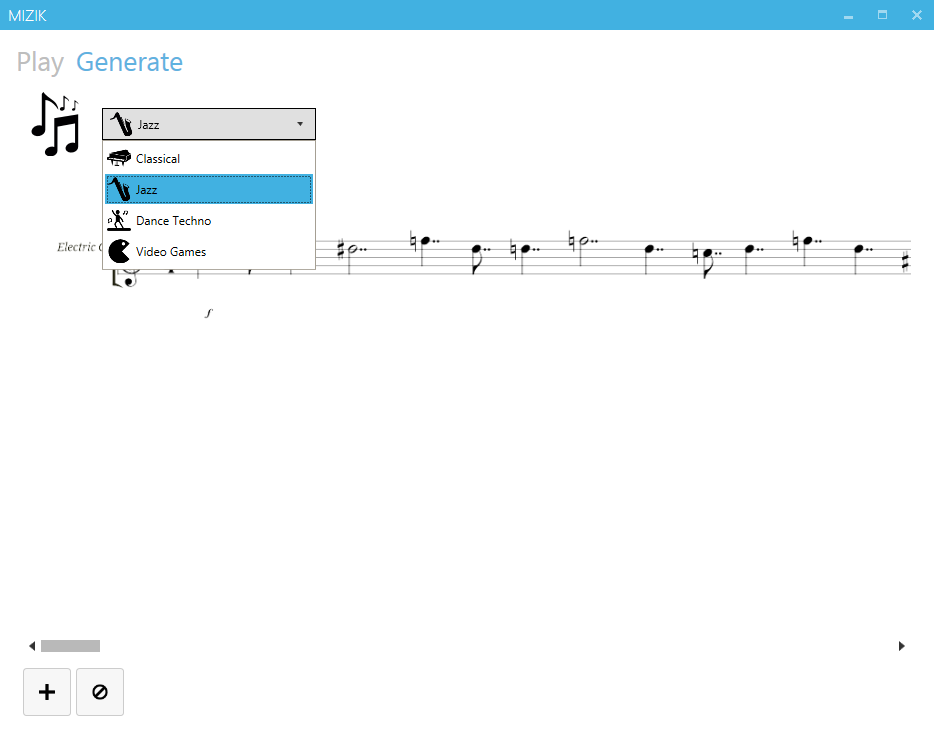
\includegraphics[width=400px]{../images/res_ui_generate_tab.png}}
\caption{Playback tab of main window}
\label{ims:res_ui_generate}
\end{figure}

Figure \ref{ims:res_ui_generate} shows composition tab of the main window. The visualization shows the current composition. A new track can be added to the composition on which the track generator window is shown. 
In addition a context menu provides the following features:
\begin{itemize}
\item Modification of the tempo of a track
\item Modification of the tempo of a track
\item Ability to show the frequency metrics of the current track
\end{itemize}

As can be seen from the figures the user interface features a clean, simple and friendly design that is based on the Metro style in Windows.


\section{Algorithms}
As has been previously mentioned the results of the algorithms were discussed in part \ref{part:algo}.
Some modification and changes were made. Most significantly the parameters of the algorithms can be modified by using the track generator. This provides some flexibility to the user.

In addition a random walk algorithm was implemented. This algorithm randomly walks through the selected scale. Although the algorithm does not compose music in a certain style and is quite simple and repetitive it does provide a useful comparison and can be used to generate simple melodies.

Some interesting melodies were produced throughout. Figure \ref{ims:res_melody_bass_drum} shows an excerpt of a melody containing acoustic bass and percussion instruments which play well together. Figure \ref{ims:res_melody_string_spacey} is a melody with a string ensamble which has a deep and spacey feel. Figure \ref{ims:res_melody_trumpet_drum} is a melody containing a trumpet and drums in a very Jazz vibe.

\begin{figure}
\centerline{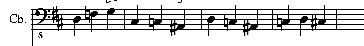
\includegraphics[width=300px]{../images/res_melody_bass_drum.pdf}}
\caption{Excerpt of a melody with acoustic bass and percussion}
\label{ims:res_melody_bass_drum}
\end{figure}

\begin{figure}
\centerline{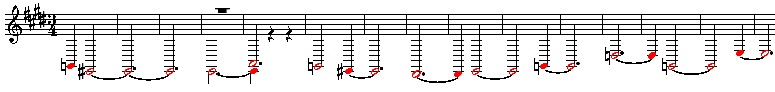
\includegraphics[width=300px]{../images/res_melody_spacey_string.pdf}}
\caption{Excerpt of a melody with a string ensamble}
\label{ims:res_melody_string_spacey}
\end{figure}

\begin{figure}
\centerline{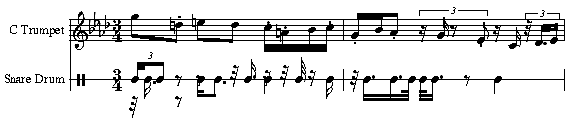
\includegraphics[width=300px]{../images/res_melody_trumpet_drum.pdf}}
\caption{Excerpt of a melody with a trumpet and drum}
\label{ims:res_melody_trumpet_drum}
\end{figure}

Overall some instruments did better than others. Especially with the Markov models, however this might be due to the input data. 

Some interesting subjective observations made include:
\begin{enumerate}
\item The trumpet in the Jazz style performed well in most algorithms
\item The violin performed poorly
\item Jazz generation all round produced more pleasant melodies
\item Classical produced average results. Classical contained a mixture of classical music. It would be interesting to see how the algorithms performed on a subset of classical music, for example on Bach's music
\item Video game music produced interesting music especially background music, for example for use in video games, or elevators or similar applications.
\item More work is required in accompaniment generation. For longer pieces the tracks desynchronize.
\end{enumerate}

\chapter{Conclusion}
The aim of this project was to design an application that is able to compose melodies in a certain musical style using machine learning algorithms. A brief survey was done on existing attempts to compose melodies using machine learning techniques.
\\

Evolutionary algorithms are versatile and are well suited to the the task of musical composition. The task of designing a good fitness function for a genetic algorithm is rather formidable.
Musical composition is a emotional human process and is subjective in nature. This makes formalization of what constitutes a good melody difficult. 
An attempt was made by using the \ac{NCD} to rate the fitness of melodies, however the results were not satisfactory.
Decent results were obtained by using frequency metrics in conjuction with a similarity measure. This approach provides high fitness to individuals which have similar statistical properties to the target piece. The problem with the approach is that a high statistical similarity may be achieved but this does not necesarily imply that a individual will be perceived as pleasant or good.
\\

A different approach was taken thereafter, other than relying on statistical properties and requiring a function to quantify the pleasantness of a melody. A probalistic approach was taken to predict the pattern of melodies. By employing the Markov property - the probability distribution of future states depend only upon the present states simplifications can be made and Markov Models can be designed. The simplest Markov Model, the Markov Chain produced pleasant results. A third order Markov Chain, where the next note is determined by the preceeding 3 notes produced pleasant results without sacrificing too much novelty and avoiding too much similarity. By employing another Markov Model, attempt was made to produce an accompaniment for a melody, by calculating the probilities for an accompaniment note by the preceeding 2 notes in the melody track. This Markov Model also yielded satisfactory results however more work is required on timing and synchronization.
Overall these probalistic models yield good results, however the melodies produce lack an overarching theme and structure. Furthermore since Markov Models require a input dataset in order to calculate the state transition and observation emission probabilities, the novelty and composition value are low. These models produce pleasant results but are not creative or original. This is in contrast to the evolutionary algorithms.
\\

Further works is needed to develop an algorithm that is able to compose melodies that have an overarching theme or structure.  Further work can be done using recurrent neural networks in a variety of topologies or using a custom \ac{HMM} that is designed for a single musical style. 
These two techniques were used in a simplistic way to generate the accompaniment to a melody with acceptable results, however these models are powerful and further work can be done.
\\

The results of most the algorithms could be improved by incorporating domain knowledge into the system. Musical knowledge could constrain the algorithm to produce more acceptable results. A hybrid system that incorporates expert knowledge may reduce the number of unpleasant patterns produced and improve note transitions and so forth.
\\

The application used a number of simplifications. A major simplification was that only monophonic melodies were considered, no chords. A more advanced system can be designed that applies the investigated algorithms to chords as well. Further algorithms could be used for harmonization.
\\

The application conforms to the specifications and is able to satisfactorily produce melodies in Classical, Jazz, Drum and Video Games styles using Markov Models, Neural Networks and Genetic Algorithms.

\chapter{Future Work}

In this chapter some ideas for future work on the application are summarized.
The ideas for future work include:

\begin{itemize}
\item If the application is to be used for background application let the algorithms generate piece of infite length and continously play the melodies.
\item Further work is required on accompaniment generation.
\item Classical music can be split into multiple sub categories. One idea is to have a different style for each famous composer.
\item Support for chords and polyphonic melodies. Algorithms can be extended to support this.
\item Further work can be done using recurrent neural networks for melody generation rather than accompaniment generation.
\item The algorithmic music composition field is large. There are a multitude of other algorithms which can be implemented.
\item Better datasets can be used. Each individual \ac{MIDI} file can be reviewed for inclusion.
\end{itemize}